\section{Training Dynamics for Multi-Step Prediction}
\label{sec:training-evolution}

\subsection{Baseline: single-step teacher forcing (V5)}

The V5 model is trained with plain single-step supervision: at every
optimization step, the model observes the ground-truth frame at time $t$
and is trained (binary cross-entropy with label smoothing $\varepsilon=0.1$)
to predict the ground-truth frame at $t+1$. This is standard \emph{teacher
forcing} and never exposes the model to its own prediction errors during
training.

V5 reaches strong single-step metrics (best validation loss $0.20125$,
precision $99.4\%$, recall $99.7\%$), but per-event accuracy reveals a
weakness: \emph{born} accuracy (correctly predicting a birth, i.e.\
dead$\to$alive) is only $93.8\%$, well below \emph{survival} accuracy
($99.8\%$) and \emph{death} accuracy ($99.9\%$). When the trained model is
unrolled autoregressively (feeding its own prediction back in as the next
input, rather than the ground truth), sparse configurations tend to
collapse to the all-dead state after a handful of steps: because the model
was never trained on grids containing its own error patterns, occasional
missed births are never corrected and instead compound, until the local
neighborhood has too few live cells to sustain any further births. This is
the classic \emph{exposure bias} problem for autoregressive sequence models.

\begin{figure}[htbp]
  \centering
  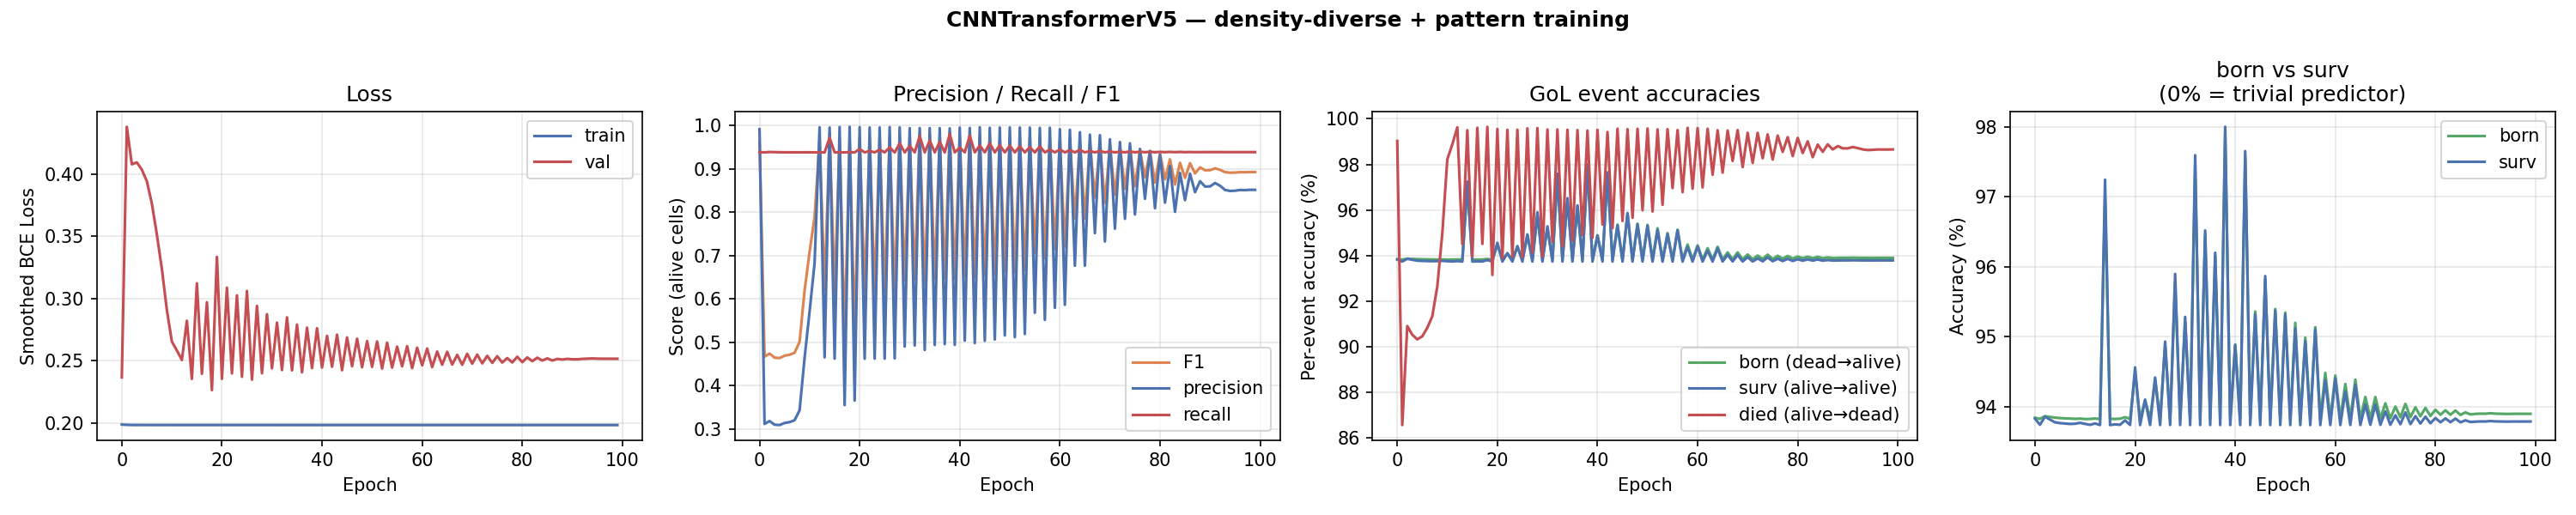
\includegraphics[width=0.85\textwidth]{figures/v5_loss.png}
  \caption{V5 training curves (single-step teacher forcing). Aggregate
  metrics look strong, but this model still collapses under
  autoregressive rollout on sparse grids.}
  \label{fig:v5-loss}
\end{figure}

\subsection{Failed fix: straight-through estimator multi-step training (V6)}

To directly train for rollout stability, V6 unrolls the model for $K=3$
steps during training. At each step, the model's \emph{hard} (binarized)
prediction is fed forward as the next input, while gradients are passed
back through the \emph{soft} (sigmoid) prediction via a straight-through
estimator (STE) --- i.e., $\text{forward} = \mathbb{1}[\sigma(x) > 0.5]$,
$\text{backward} = \nabla \sigma(x)$.

V6 performs well only transiently: at epoch 5 (warm-started from V5) it
reaches validation loss $0.23421$ with precision $92.7\%$ and born-accuracy
$99.5\%$, but precision then collapses to $20$--$50\%$ over the following
epochs and oscillates chaotically through epoch 50 (Figure~\ref{fig:v6-loss}).
Gradient clipping (already active at $\text{max\_norm}=1.0$) does not
resolve this. We hypothesize the failure mode is a \emph{systematic
directional gradient bias}: when the model misses a birth at step $t$, step
$t+1$'s input is missing a live cell relative to ground truth, and the STE
gradient at step $t+1$ consistently signals ``predict more alive'' back
through the network, regardless of whether more alive cells are actually
correct at $t$. This creates a positive-feedback loop toward over-predicting
liveness that is not a magnitude problem (which clipping could fix) but a
\emph{direction} problem.

\begin{figure}[htbp]
  \centering
  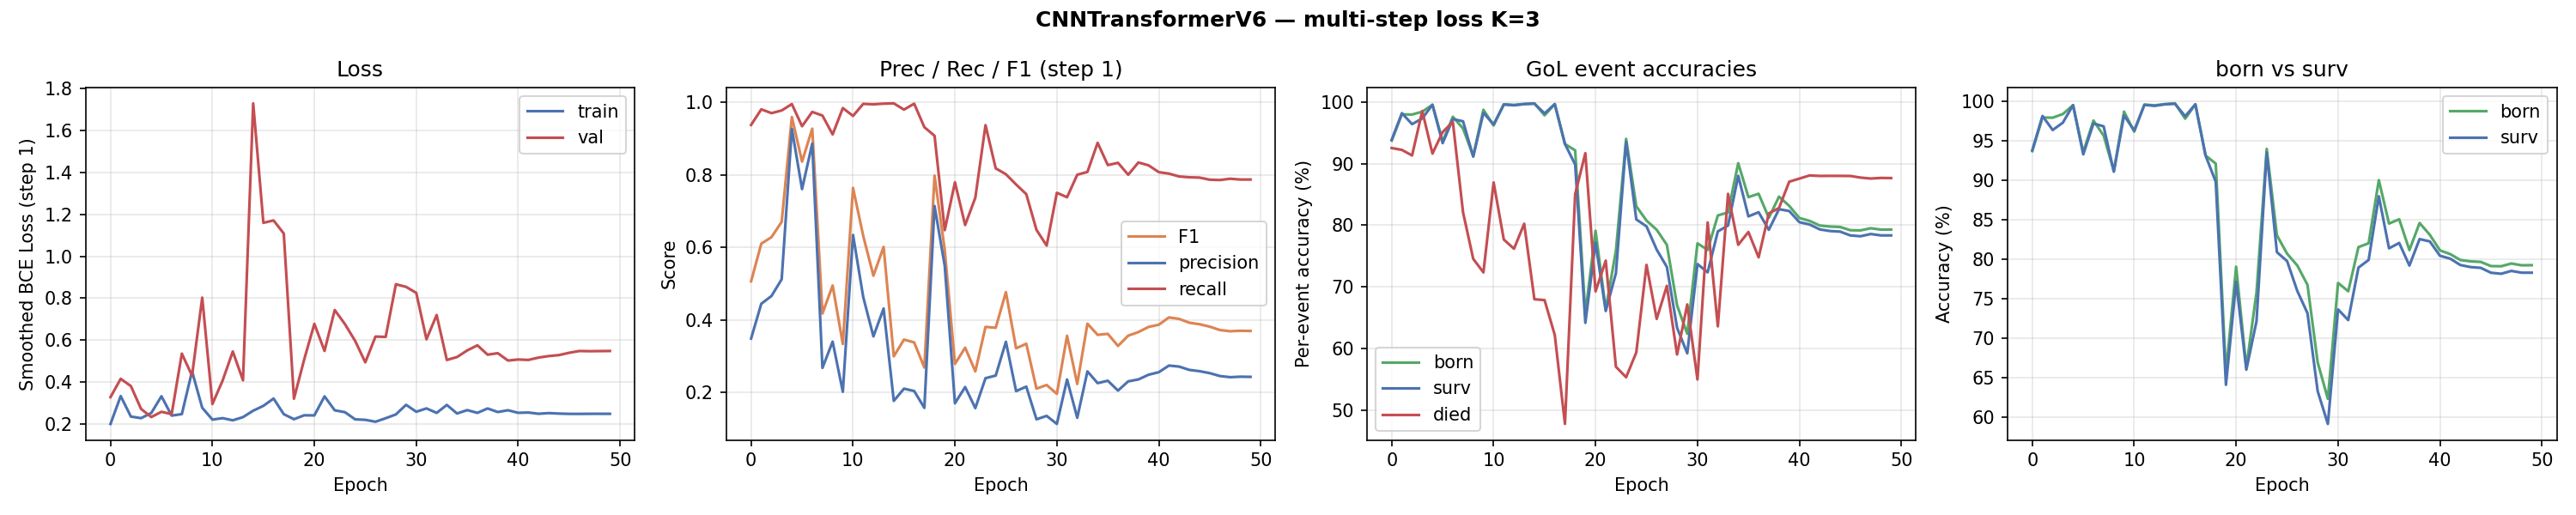
\includegraphics[width=0.85\textwidth]{figures/v6_loss.png}
  \caption{V6 training curves (STE multi-step, $K=3$). Precision collapses
  after an initial promising region around epoch 5 and never recovers.}
  \label{fig:v6-loss}
\end{figure}

A second attempt with STE at a lower learning rate ($1\mathrm{e}{-5}$) and
$K=2$ still diverged, with the same directional signature (precision
falling monotonically from epoch 1 to epoch 5), confirming the bias is
intrinsic to the STE gradient path rather than an optimization-stability
artifact.

\subsection{Working fix: scheduled sampling (V7)}

V7 replaces the STE hard/soft split with \emph{scheduled sampling}
\cite{bengio2015scheduled}: at each of the $K=3$ unrolled steps, the next
input is the model's own (hard, binarized) prediction with probability
$p$, or the ground-truth frame with probability $1-p$, where $p$ increases
linearly from $0$ to $1$ over training. Critically, gradients flow only
through the \emph{current} step's logits --- there is no gradient path
connecting step $t+1$'s loss back to step $t$'s prediction, which removes
the STE's compounding directional bias entirely.

V7 trains stably for all 50 epochs (Figure~\ref{fig:v7-loss}) and reaches
the best aggregate metrics of any single-step-warm-started model in this
study: validation loss $0.20114$, F1 $0.9985$, precision $99.7\%$, recall
$100\%$, and \emph{all three} per-event accuracies (born, survival, death)
at $99.7$--$100\%$. Qualitatively, the artifact of rollouts settling into
sparse grid-aligned dead patterns --- visible in V5/V6 rollouts on sparse
inputs --- disappears entirely.

\begin{figure}[htbp]
  \centering
  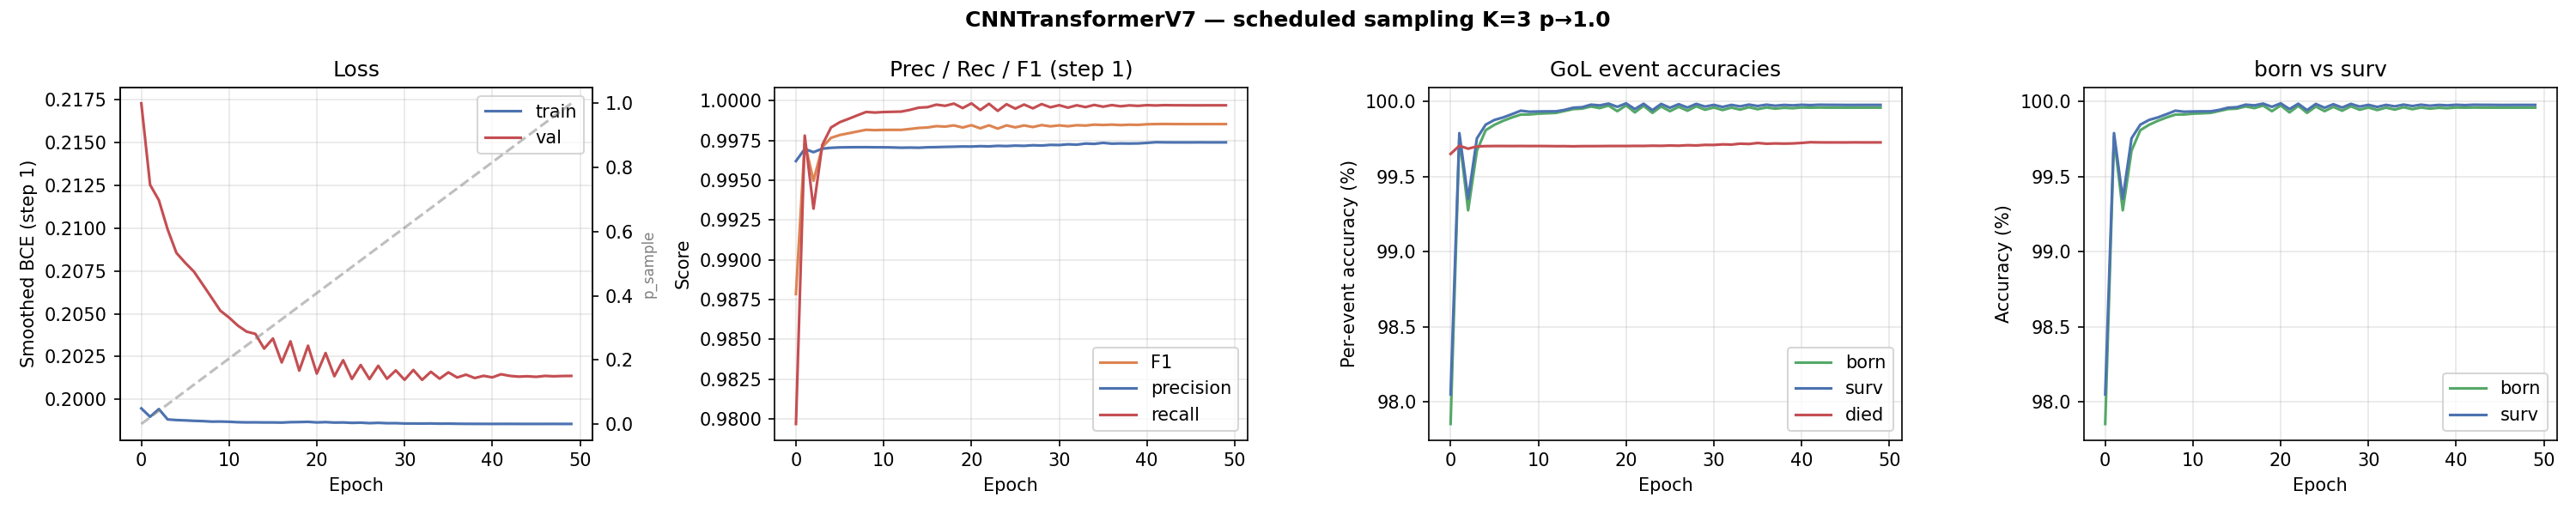
\includegraphics[width=0.85\textwidth]{figures/v7_loss.png}
  \caption{V7 training curves (scheduled sampling, $K=3$, $p: 0\to1$).
  Training is stable across all 50 epochs, with monotonically improving
  per-event accuracies.}
  \label{fig:v7-loss}
\end{figure}

\subsection{Targeted fine-tuning at high density (V8)}

Although V7's aggregate metrics are strong, a targeted failure search
(random grids across densities $0.02$--$0.80$, and 8 named small patterns,
seed-matched for reproducibility) finds that essentially all remaining
errors concentrate at high density ($d=0.80$), with roughly $100$ false
positives per grid on average.

V8 continues training V7's checkpoint for 30 further epochs with a dataset
that upsamples $d=0.65$ and $d=0.80$ trajectories by $3\times$ relative to
V7's dataset, while retaining the full range of lower densities (so the
model does not lose accuracy on sparse/medium configurations it already
handles well). This reduces the mean false-positive count at $d=0.80$ from
approximately $100$/grid to approximately $4.6$/grid --- a
$21\times$ improvement --- while aggregate metrics improve marginally
(validation loss $0.20064$, precision $100\%$, recall $99.9\%$).
Figure~\ref{fig:v7-v8-compare} shows a direct comparison of V7 and V8 on
one of the exact failure grids identified in the V7 failure search.

\begin{figure}[htbp]
  \centering
  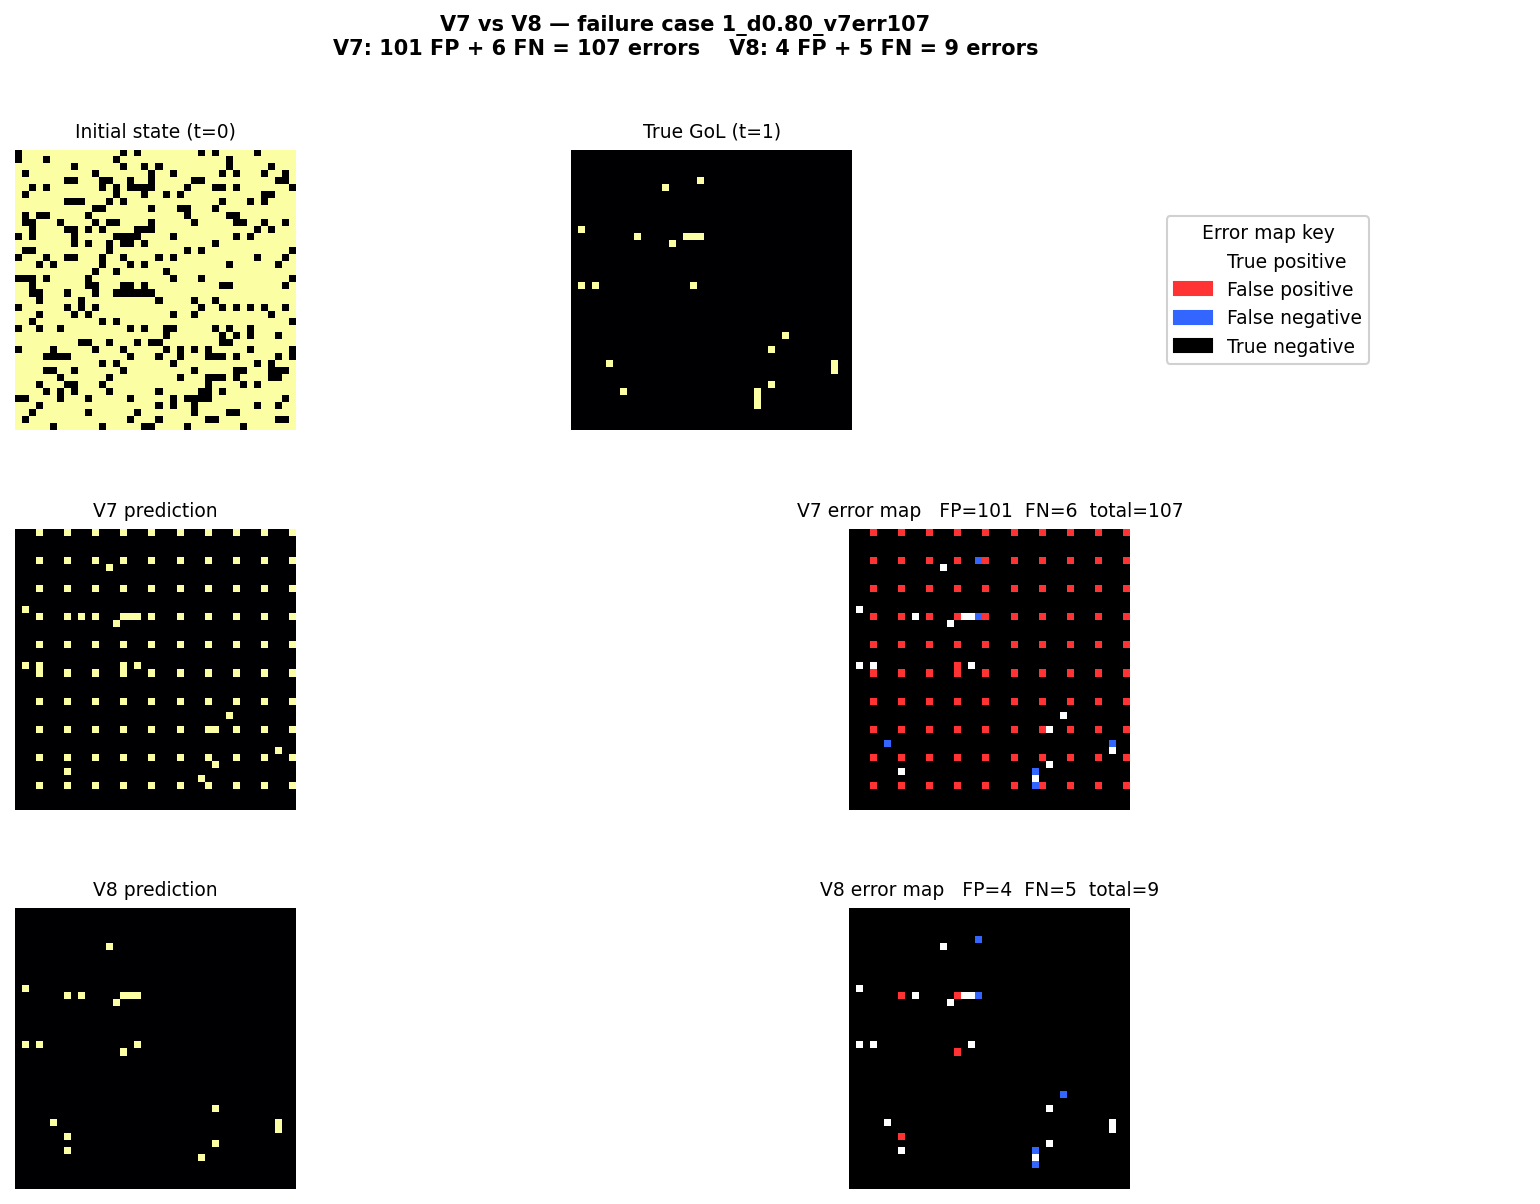
\includegraphics[width=0.95\textwidth]{figures/v7_v8_failure_compare.png}
  \caption{V7 vs.\ V8 on an identical $d=0.80$ failure grid found during the
  V7 failure search. V7 makes 107 errors (mostly false positives, visible as
  a diffuse grid-aligned speckle pattern); V8, fine-tuned with $3\times$
  more high-density data, makes substantially fewer errors on the same
  input.}
  \label{fig:v7-v8-compare}
\end{figure}

\subsection{Data scale-up regresses performance (V9)}

Given V8's improvement from more high-density data, we test whether scaling
\emph{all} data five-fold (approximately $546{,}200$ total training
examples, warm-started from V8) improves matters further. Aggregate
validation metrics remain similar to V8 (validation loss $0.20118$,
precision $99.7\%$, recall $99.6\%$), but per-grid error counts on the same
failure-search protocol \emph{worsen substantially}: false positives at
$d=0.80$ increase from V8's $2{,}296$ (across 500 grids) to $22{,}190$, and
false negatives at $d=0.50$ increase from $67$ to $6{,}948$.

This is the central negative result motivating Section~\ref{sec:results-table}:
\emph{aggregate validation metrics can look stable even as tail-case
behavior regresses sharply}, and simply scaling the training set does not
help once a model has saturated its representational capacity --- indeed it
can actively hurt, plausibly because the effective gradient signal from
over-represented high-density trajectories (each contributing many
alive-cell examples) skews optimization away from the sparse/medium regime
that was previously well-fit.

\begin{figure}[htbp]
  \centering
  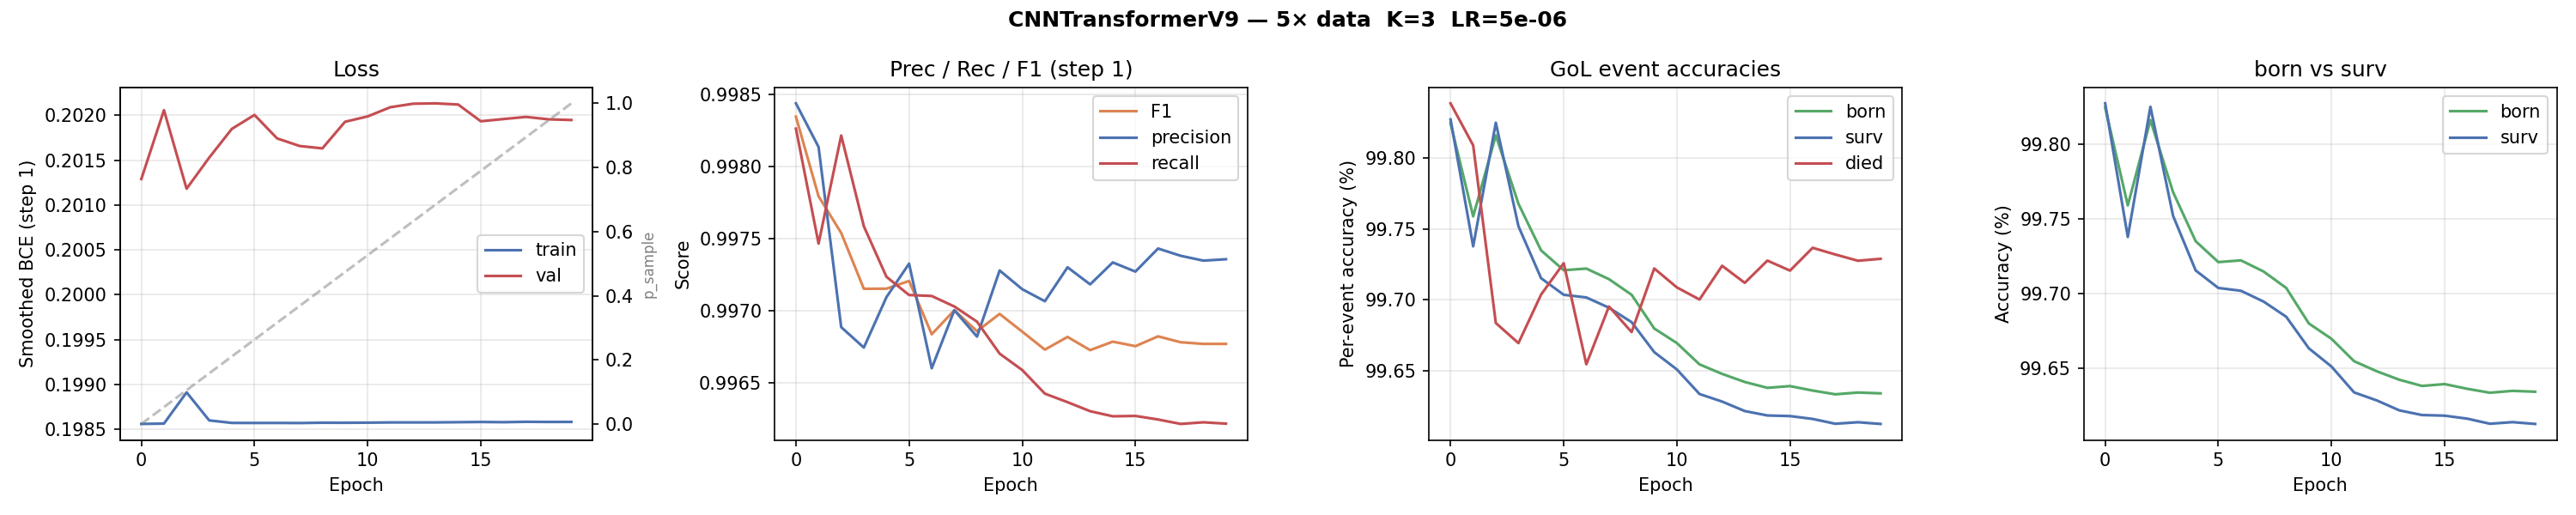
\includegraphics[width=0.85\textwidth]{figures/v9_loss.png}
  \caption{V9 training curves (5$\times$ data scale-up, warm-started from
  V8). Aggregate metrics look unremarkable, masking a substantial
  regression in per-grid tail-case error counts (see
  Table~\ref{tab:version-summary}).}
  \label{fig:v9-loss}
\end{figure}

\subsection{Scaling model capacity instead (V10)}

Rather than scaling data further, V10 scales the \emph{model}: doubling
$d_{\text{model}}$ ($64\to128$), doubling attention heads ($4\to8$), and
adding two Transformer layers ($4\to6$), for a total of $1{,}504{,}240$
parameters (5.15$\times$ V8's size). Because the embedding dimension
changes, V10 is trained \emph{from scratch} (V8/V9's weights cannot be
warm-started into a different-width model) using the same scheduled
sampling recipe and V8's dataset configuration (i.e., \emph{not} the 5$\times$
scaled-up V9 dataset).

V10 converges essentially immediately: by epoch 10 of 100, all metrics
(precision, recall, born, survival, death) reach $100.0\%$ and validation
loss reaches $0.19852$ --- notably \emph{below} the theoretical
label-smoothing floor achieved by any previous version, and the model
holds this exactly through epoch 100 (Figure~\ref{fig:v10-loss}).

\begin{figure}[htbp]
  \centering
  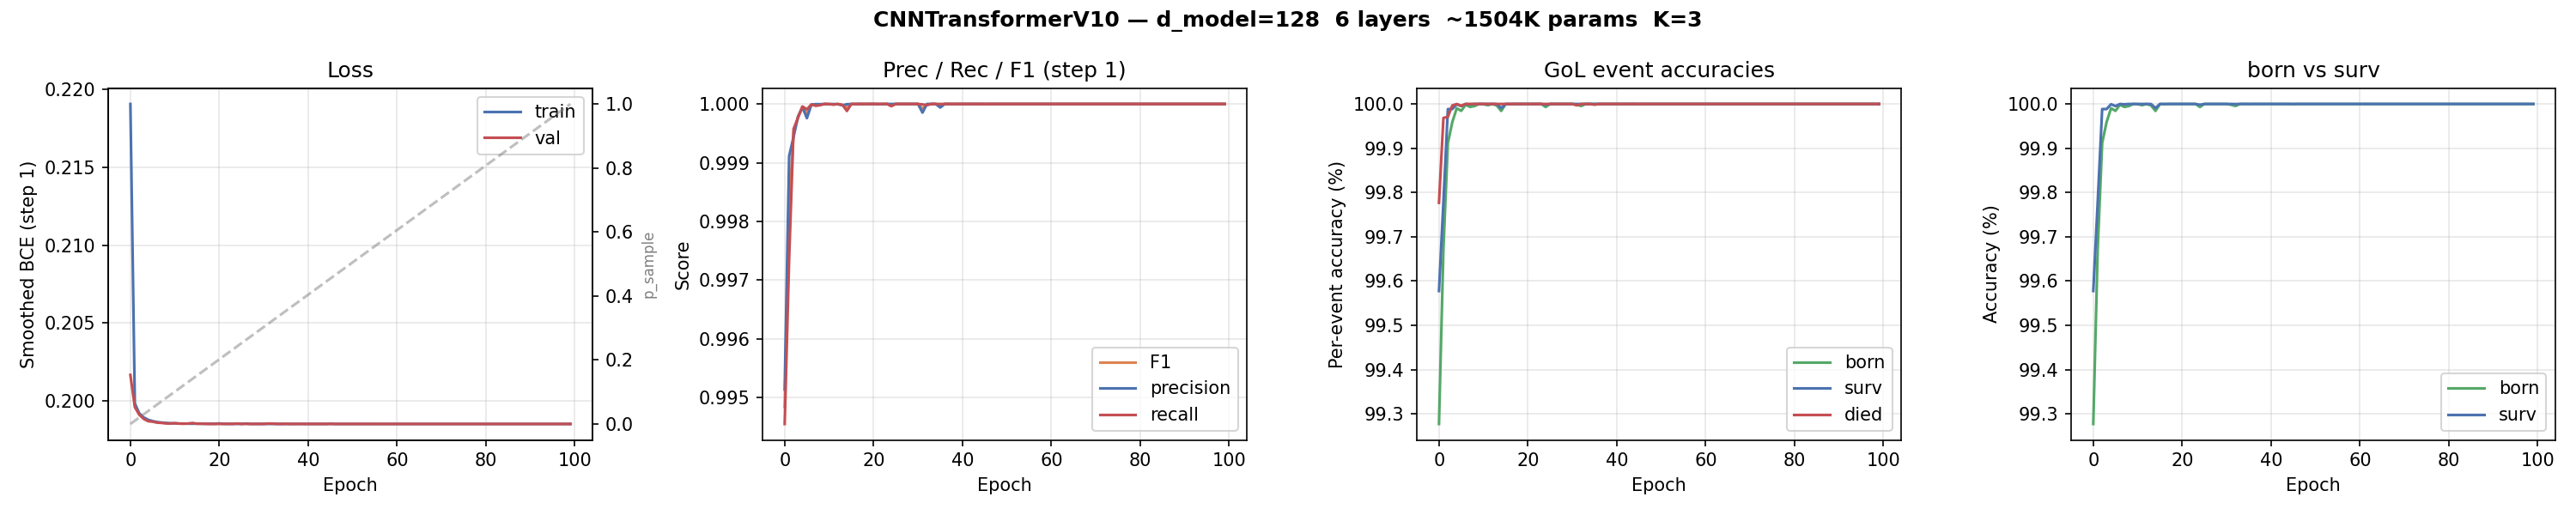
\includegraphics[width=0.85\textwidth]{figures/v10_loss.png}
  \caption{V10 training curves ($d_{\text{model}}=128$, 6 layers,
  $1.5$M params, trained from scratch). All metrics saturate at $100\%$
  by epoch 10 and remain stable through epoch 100.}
  \label{fig:v10-loss}
\end{figure}

Repeating the exact per-grid failure-search protocol used for V8/V9 (500
grids per density, densities $0.20$--$0.80$, fixed seed), V10 makes
\textbf{zero errors across all 2{,}500 evaluated grids} --- a qualitative
change from V8's thousands of residual errors at high density
(Table~\ref{tab:version-summary}, Figure~\ref{fig:v10-rollout}).

\begin{figure}[htbp]
  \centering
  \begin{subfigure}[t]{0.48\textwidth}
    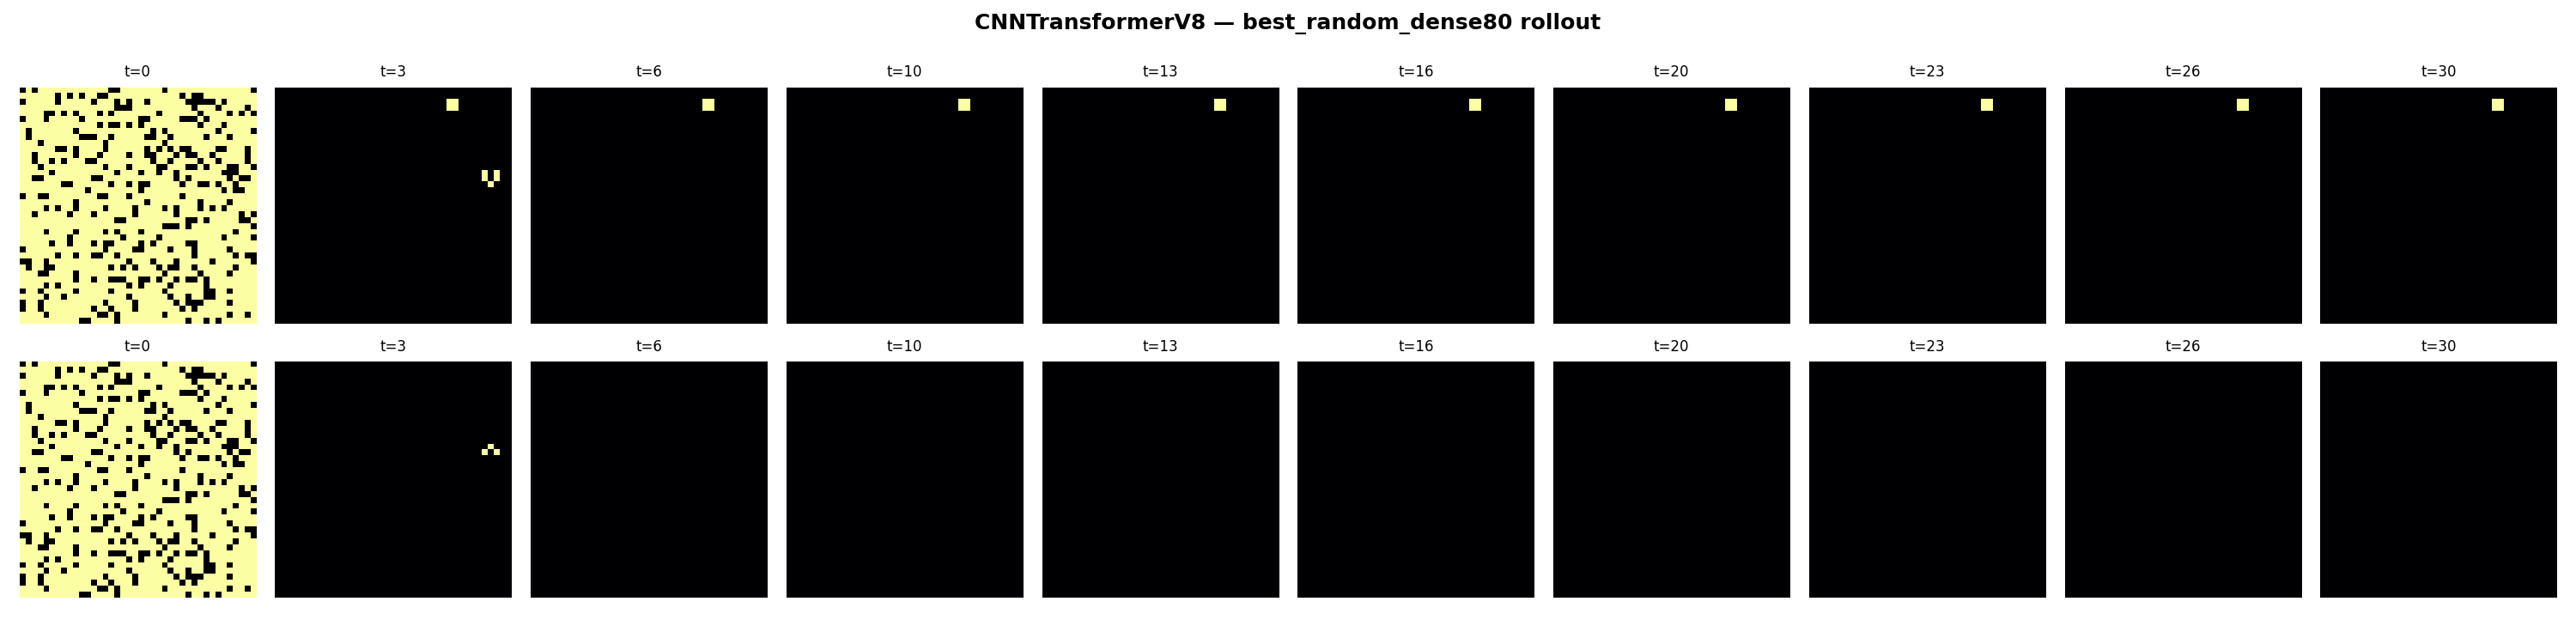
\includegraphics[width=\textwidth]{figures/v8_rollout_dense80.png}
    \caption{V8 (291K params)}
  \end{subfigure}
  \hfill
  \begin{subfigure}[t]{0.48\textwidth}
    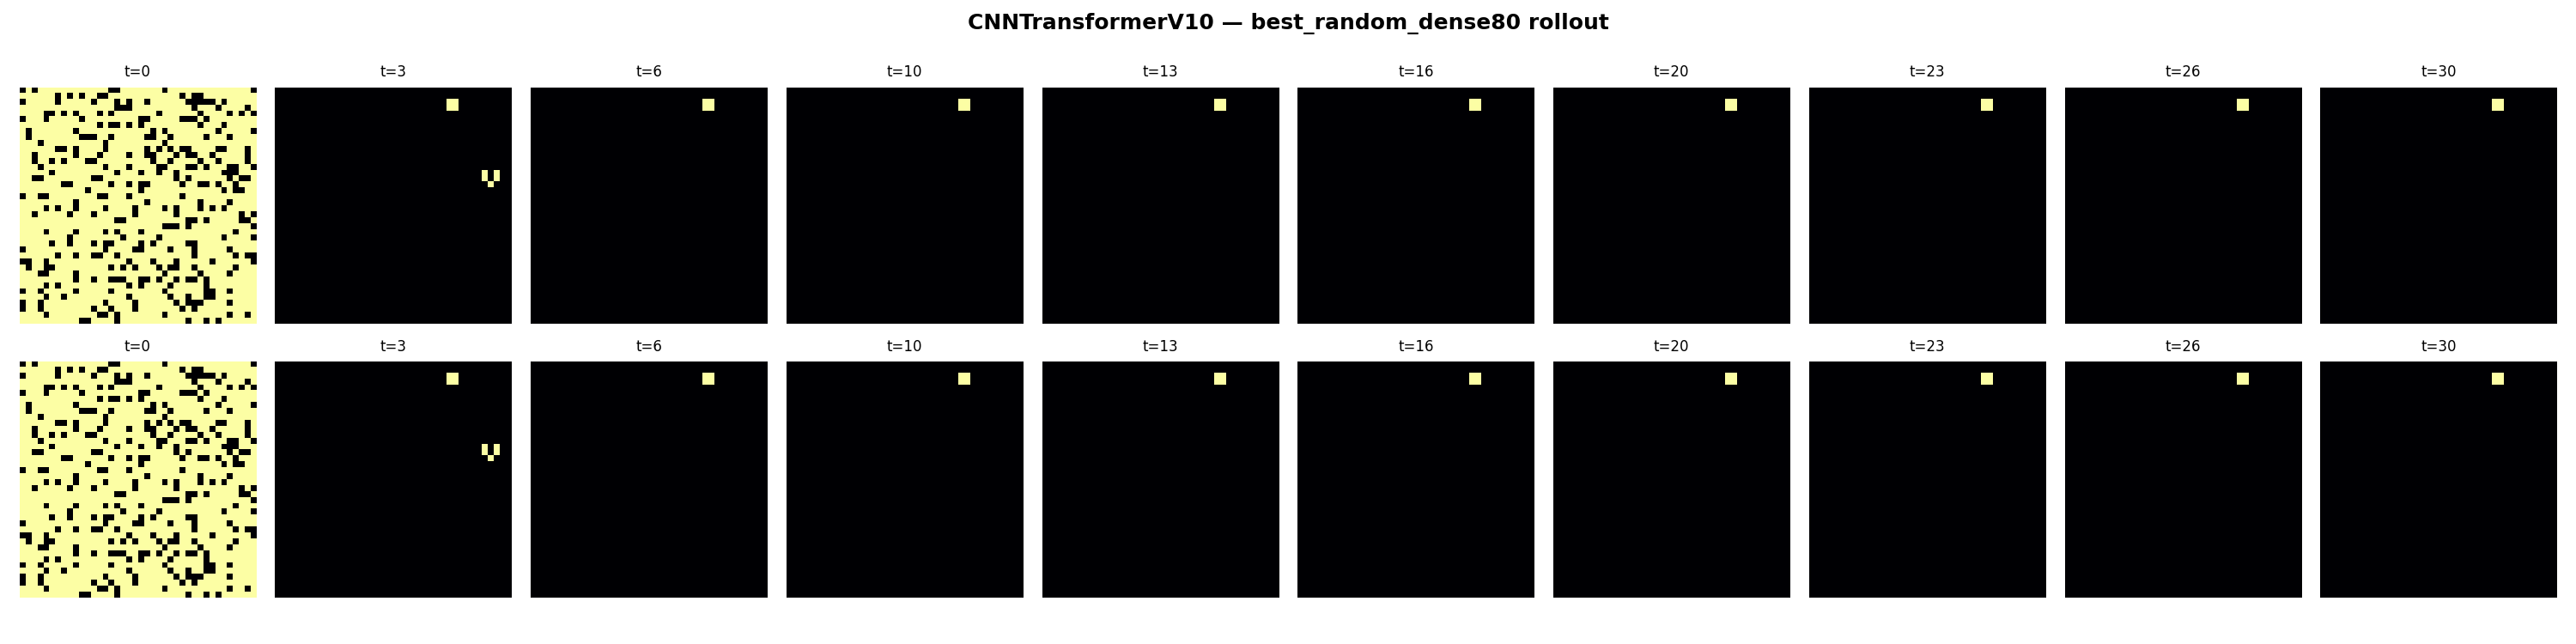
\includegraphics[width=\textwidth]{figures/v10_rollout_dense80.png}
    \caption{V10 (1.5M params)}
  \end{subfigure}
  \caption{30-step autoregressive rollout starting from a random $d=0.80$
  grid, true GoL trajectory (top row of each panel) vs.\ model prediction
  (bottom row).}
  \label{fig:v10-rollout}
\end{figure}

Taken together, V8 through V10 demonstrate that \emph{model capacity}, not
data volume, was the binding constraint at the $291$K-parameter scale: more
data of the same kind that a saturated model already sees plenty of does
not help (and can actively hurt), while more parameters directly resolve
the remaining tail-case errors.
